\documentclass[notitlepage,11pt]{article}


% Packages
% --------
%	 Necessary
\usepackage{geometry} 						% geometry - page dimensions
\usepackage[parfill]{parskip}				% parskip - to use blank line to sep paragraphs
\usepackage{titling}						% title formatting
\usepackage{enumitem}

\usepackage{amsmath}						% AMS - math, fonts, symbols, theorem
\usepackage{amsfonts}
\usepackage{amssymb}
\usepackage{amsthm}
\usepackage{mathtools}						% mathtools - \coloneqq

\usepackage{listings}						% listings - prints source code

\usepackage{hyperref}						% hyperref - urls and things

\usepackage{tikz}							% tikz - graphs

% 	Additional
\usepackage{graphicx}						% graphicx - importing graphics from file
\usepackage{subcaption}
\captionsetup[subfigure]{labelformat=empty}
\usepackage[T1]{fontenc}
\usepackage[utf8]{inputenc}
\usepackage{helvet}
\renewcommand{\familydefault}{\sfdefault}	% change to helvetica

\usepackage{forest}							% forest - easy trees
\usepackage{tikzsymbols}					% tikzsymbols - just adds some symbols
% tikzlibrary summary: 
% tex.stackexchange.com/questions/42611/list-of-available-tikz-libraries-with-a-short-introduction/491626
\usetikzlibrary{arrows.meta}				% arrows.meta - customizable arrow tips
\usetikzlibrary{er}							% entity-relationship diagrams
\usetikzlibrary{positioning} 				% relative positioning
\usetikzlibrary{shadows}
\usetikzlibrary{shapes}

\usepackage{xcolor}							% xcolor - adds additional colors

\usepackage{marginnote}						% marginnote - see name

\usepackage{multirow}						% multirow - sort of a tabular environment of text
\usepackage{bigdelim}						% bigdelim - used with multirow once to make brackets on tables
\usepackage{array}							% array - extends arrary and tabular environment
\usepackage{makecell}						% makecell - adjust cell cizes within tabular environment

\usepackage[bottom]{footmisc}				% comment out to make footnotes not appear at bottom of page

% Customizations

\pretitle{\begin{center}\Large\bfseries}		% titling format
\posttitle{\par\end{center}\vskip 0cm}
\preauthor{\begin{center}\large}
\postauthor{\end{center}}
\predate{\par\normalsize\centering}
\postdate{\par}

\newtheoremstyle{customnumber} % name
	{}% space above
	{}% space below
	{\normalfont}% body font
	{}% indent 
	{\bfseries}% head font
	{:}% punctuation between head/body
	{ }% space after head: " " = normal whitespace
	{\thmname{#1}\thmnote{ #3}}% head format

\newtheoremstyle{named}
	{}
	{}
	{\normalfont}
	{}
	{\bfseries}
	{.}
	{ }
	{\thmnote{#3}}

\theoremstyle{customnumber}
\newtheorem*{exercise}{Exercise}

\theoremstyle{definition}
\newtheorem{defi}{Definition}

\newtheorem{ex}{Example}[section]

\theoremstyle{named}
\newtheorem*{namedtheorem}{}

\newenvironment{absolutelynopagebreak}
	{\par\nobreak\vfil\penalty0\vfilneg\vtop\bgroup}
	{\par\xdef\tpd{\the\prevdepth}\egroup\prevdepth=\tpd}
	
\newcommand{\indep}{\raisebox{0.05em}{\rotatebox[origin=c]{90}{$\models$}}}

\newcommand{\stcomp}[1]{{#1}^\complement}


\lstset{tabsize=3, numbers=left, basicstyle=\ttfamily, escapeinside=~~, xleftmargin=-1cm}
\let\origthelstnumber\thelstnumber
\makeatletter
\newcommand*\Suppressnumber{%
	\lst@AddToHook{OnNewLine}{%
		\let\thelstnumber\relax%
		\advance\c@lstnumber-\@ne\relax%
	}%
}
\newcommand*\Reactivatenumber{%
	\lst@AddToHook{OnNewLine}{%
		\let\thelstnumber\origthelstnumber%
		\advance\c@lstnumber\@ne\relax%
	}%
}
\makeatother

\title{COMP 3700 Project 2 Design}
\author{Tripp Isbell\\
	\texttt{cai0004@auburn.edu}\\
	\href{https://github.com/Carbonationalism/COMP3700}{github}}
\date{}

\geometry{margin=1in}
\setlength{\droptitle}{-1.5cm}
\pagenumbering{gobble}

\graphicspath{{./UI/}}
\setitemize{noitemsep,topsep=-2pt,parsep=-2pt,partopsep=-2pt}

\usepackage[normalem]{ulem} %for strikethrough

\begin{document}
\maketitle

\textbf{Design goals:}\\
For this project I want to separate my store design into a client system that allows logins for different users with different access privileges, and a server system that allows communication with a local database. Right now my system is a tangled mess of client/server interfaces which only access the database through the server, and interfaces which require access to the local database to function. The server is also currently set up to function as a thread of the main application (so that it too can access the local database), so my first task is to separate these out such that the server is an independent application that is the only point of access to the local database. The easiest way to accomplish that is to make my server mimic the functionality of the local data access layer. 

From there the design of the customer, product, and purchase interfaces is easy since all of the user stories are unchanged from before, the only difference is the addition of the multiple user types (admin, manager, cashier, and customer) from Assignment 4, and controlling their respective access to each of the functionalities from the previous design.

So since I want my user level design to stay the same, with the client/server implementation handled behind the scenes my use cases are pretty much the same, so here are my use cases with minor adjustments from Project 1 as well as some new use cases for the Assignment 4 login system:


	\textbf{Use Case:} Generic login use case\\
	\textbf{Actors:} admin, manager, cashier, customer\\
	\textbf{Goals:} identify the type of user logging in, and display the respective interface\\
	\textbf{stes:}
	\begin{itemize}
		\item[(1)] upon launch, the client application displays a login screen
		\item the user enters a username/password combo that matches a user in the database
		\item the system sends that info to server, the server responds with correct user type
		\item[(2)] the system displays that type's respective interface (customer UI pictured)
	\end{itemize}
\begin{figure}[h]
	\begin{subfigure}{.5\textwidth}
	\centering
	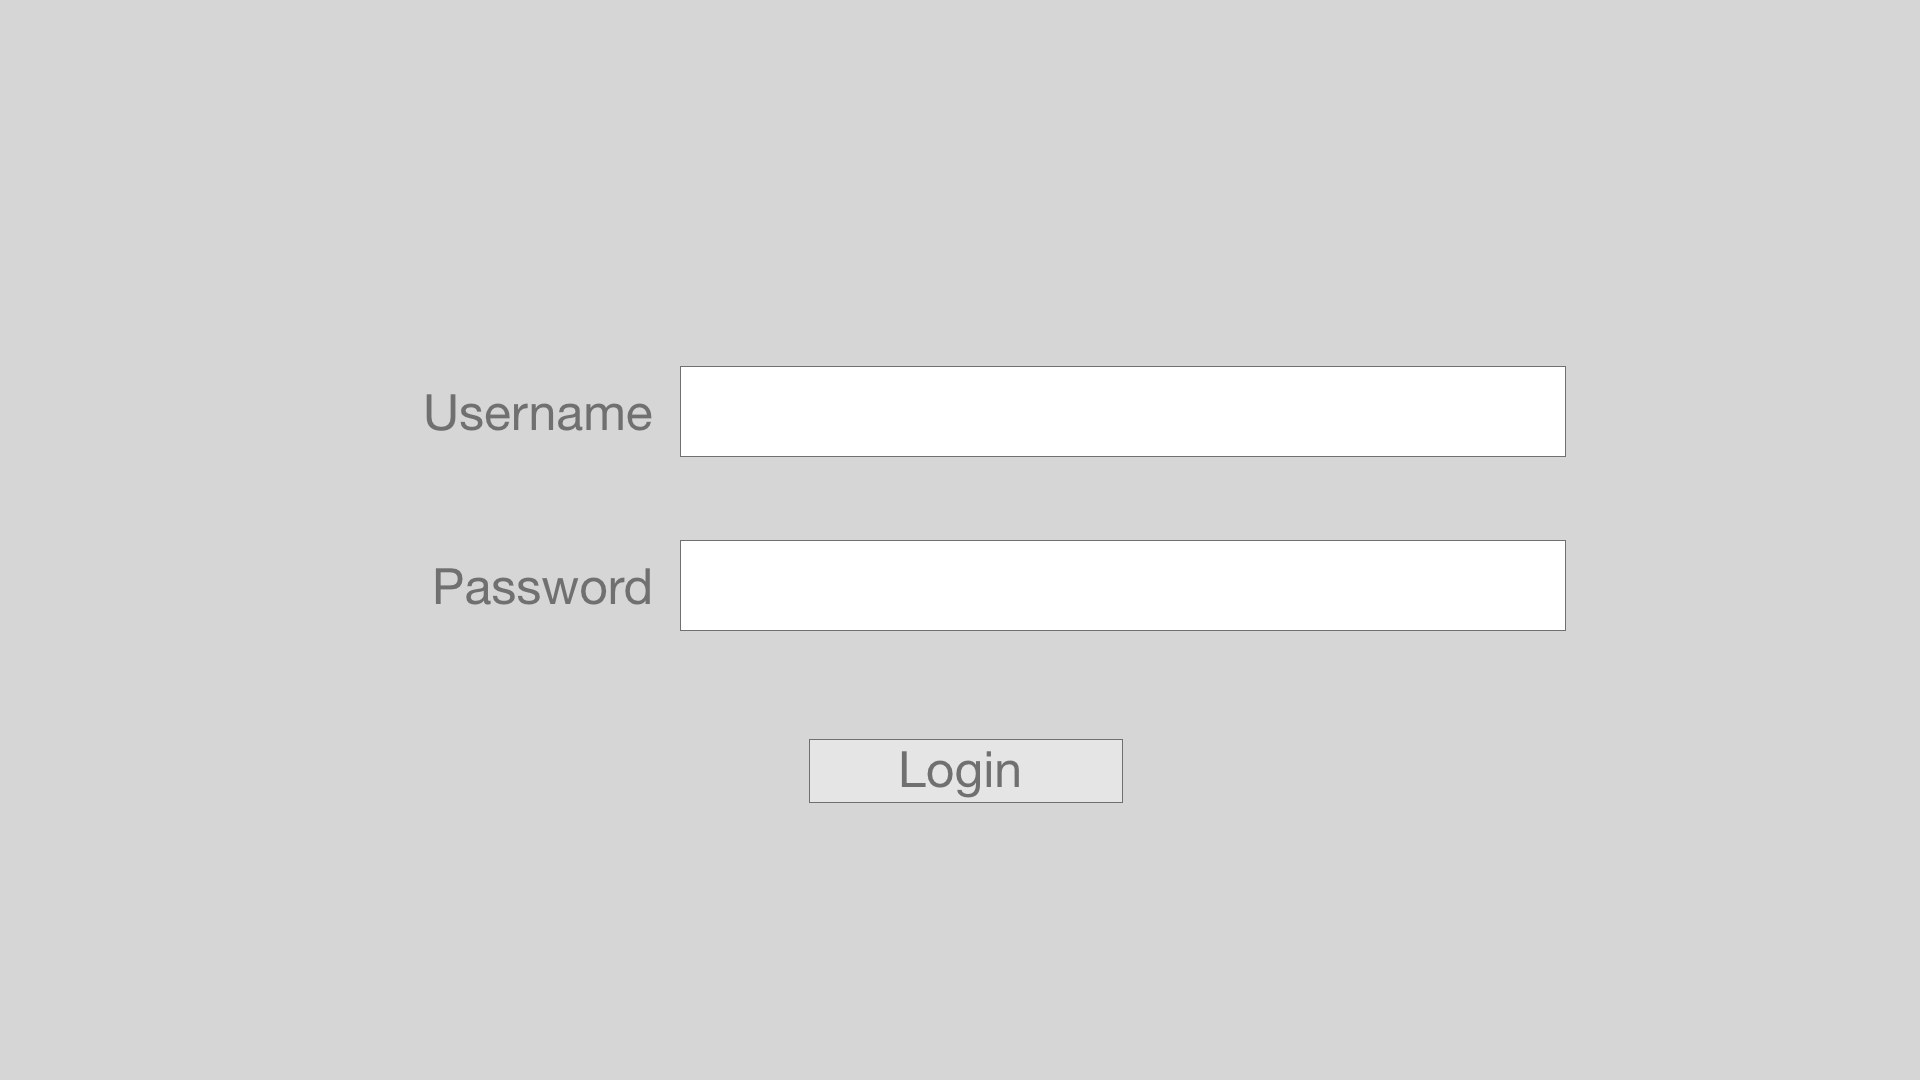
\includegraphics[scale=0.12]{LoginUI}
	\caption{(1)}
	\end{subfigure}%
	\begin{subfigure}{.5\textwidth}
	\centering
	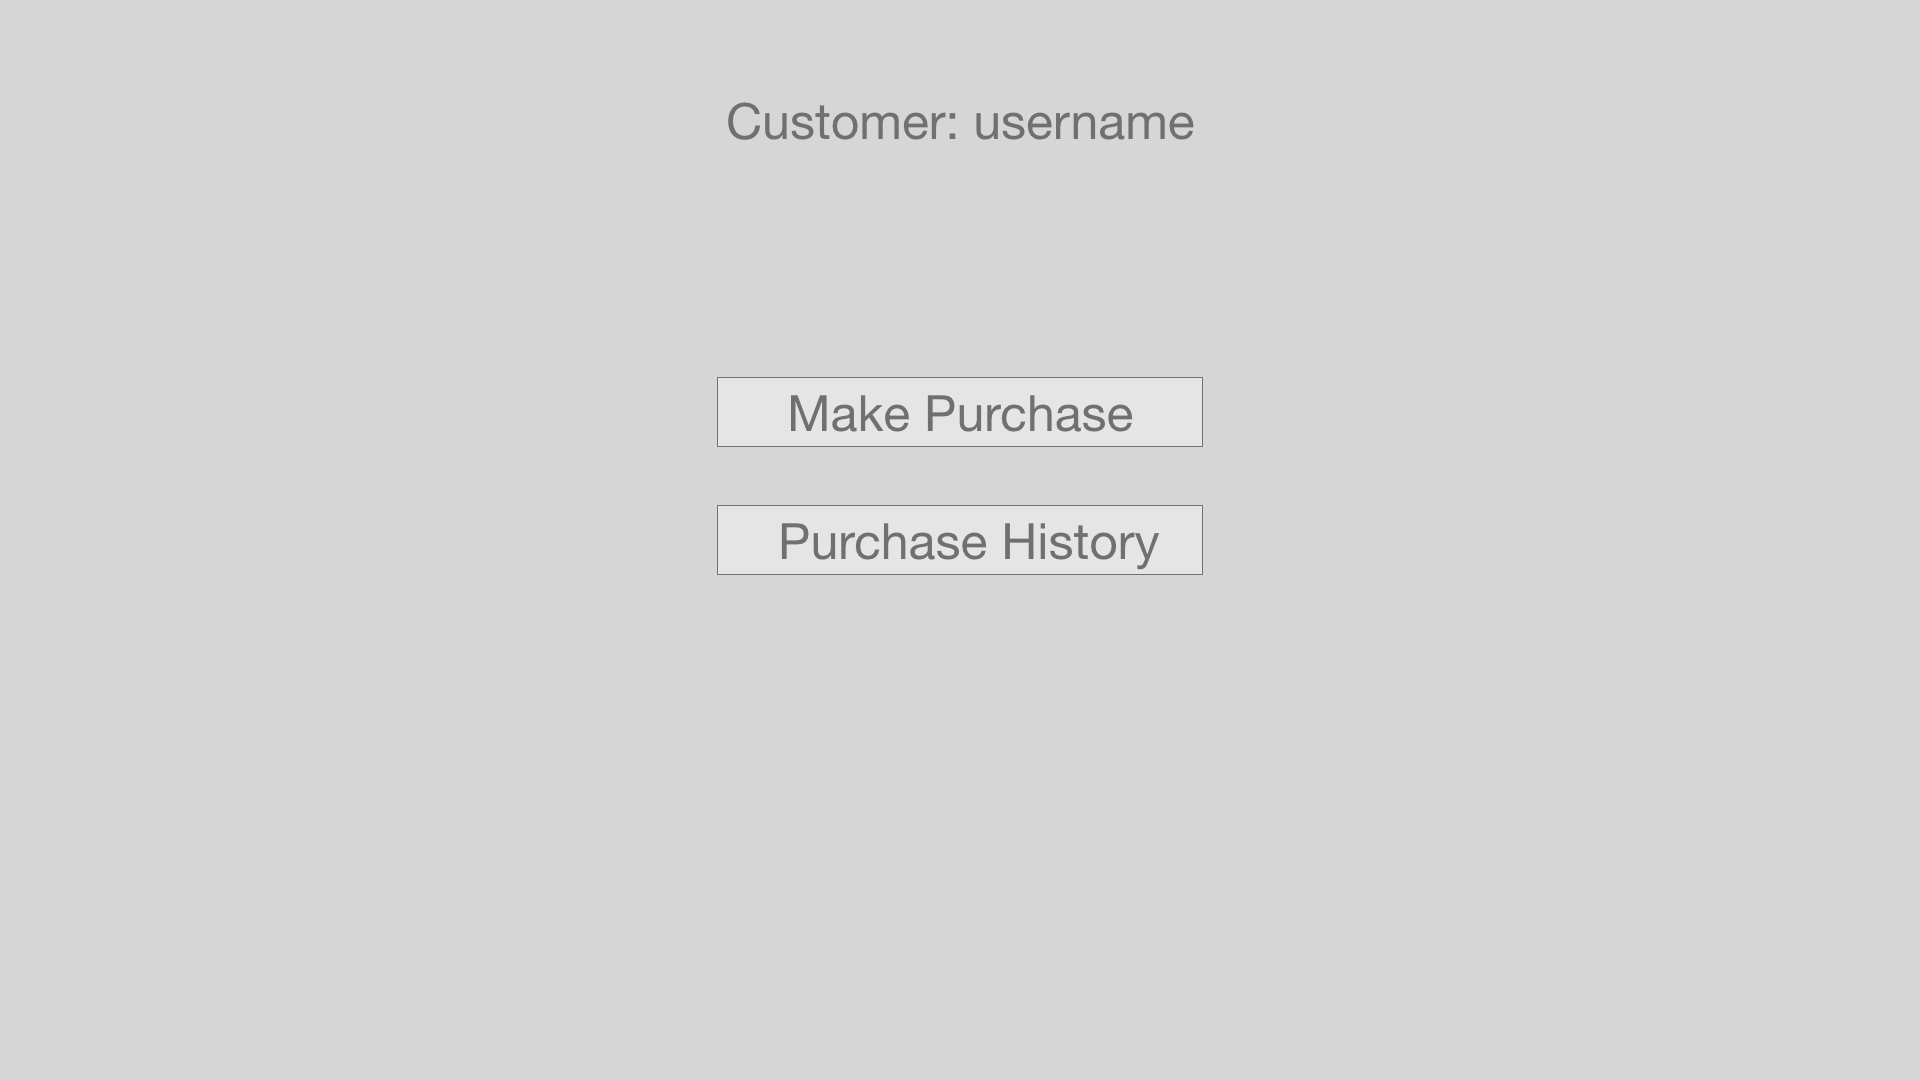
\includegraphics[scale=0.12]{CustomerUI}
	\caption{(2)}
	\end{subfigure}
\end{figure}

\section{User Story: Add Product}
\textbf{Use Case:} add a product into the system\\
	\textbf{Actors:} employees\\
	\textbf{Goals:} update database to include new product\\
	\textbf{Related use cases:} adding a customer to the database or recording a transaction (below)
	\textbf{Preconditions:} interface is functional and \sout{connected to underlying database} \emph{server is running}\\
	\textbf{Postconditions:} The product database is updated with the item\\
	\textbf{Steps:}
		\begin{itemize}
		\item[(1)] the user clicks a button to display the product database
		\item[(2)] the system \emph{fetches from server and} displays the database
		\item the user clicks add product
		\item[(3)] the system displays a screen with text fields for the product info
		\item the user enters the information and clicks an add button
		\item[(4)] the system \sout{updates the database} \emph{sends the product to server} and displays a confirmation message
		\item the user clicks confirm 
		\item[(1)] the system returns to the main menu
		\end{itemize}
\begin{figure}[h]
	\begin{subfigure}{.5\textwidth}
	\centering
	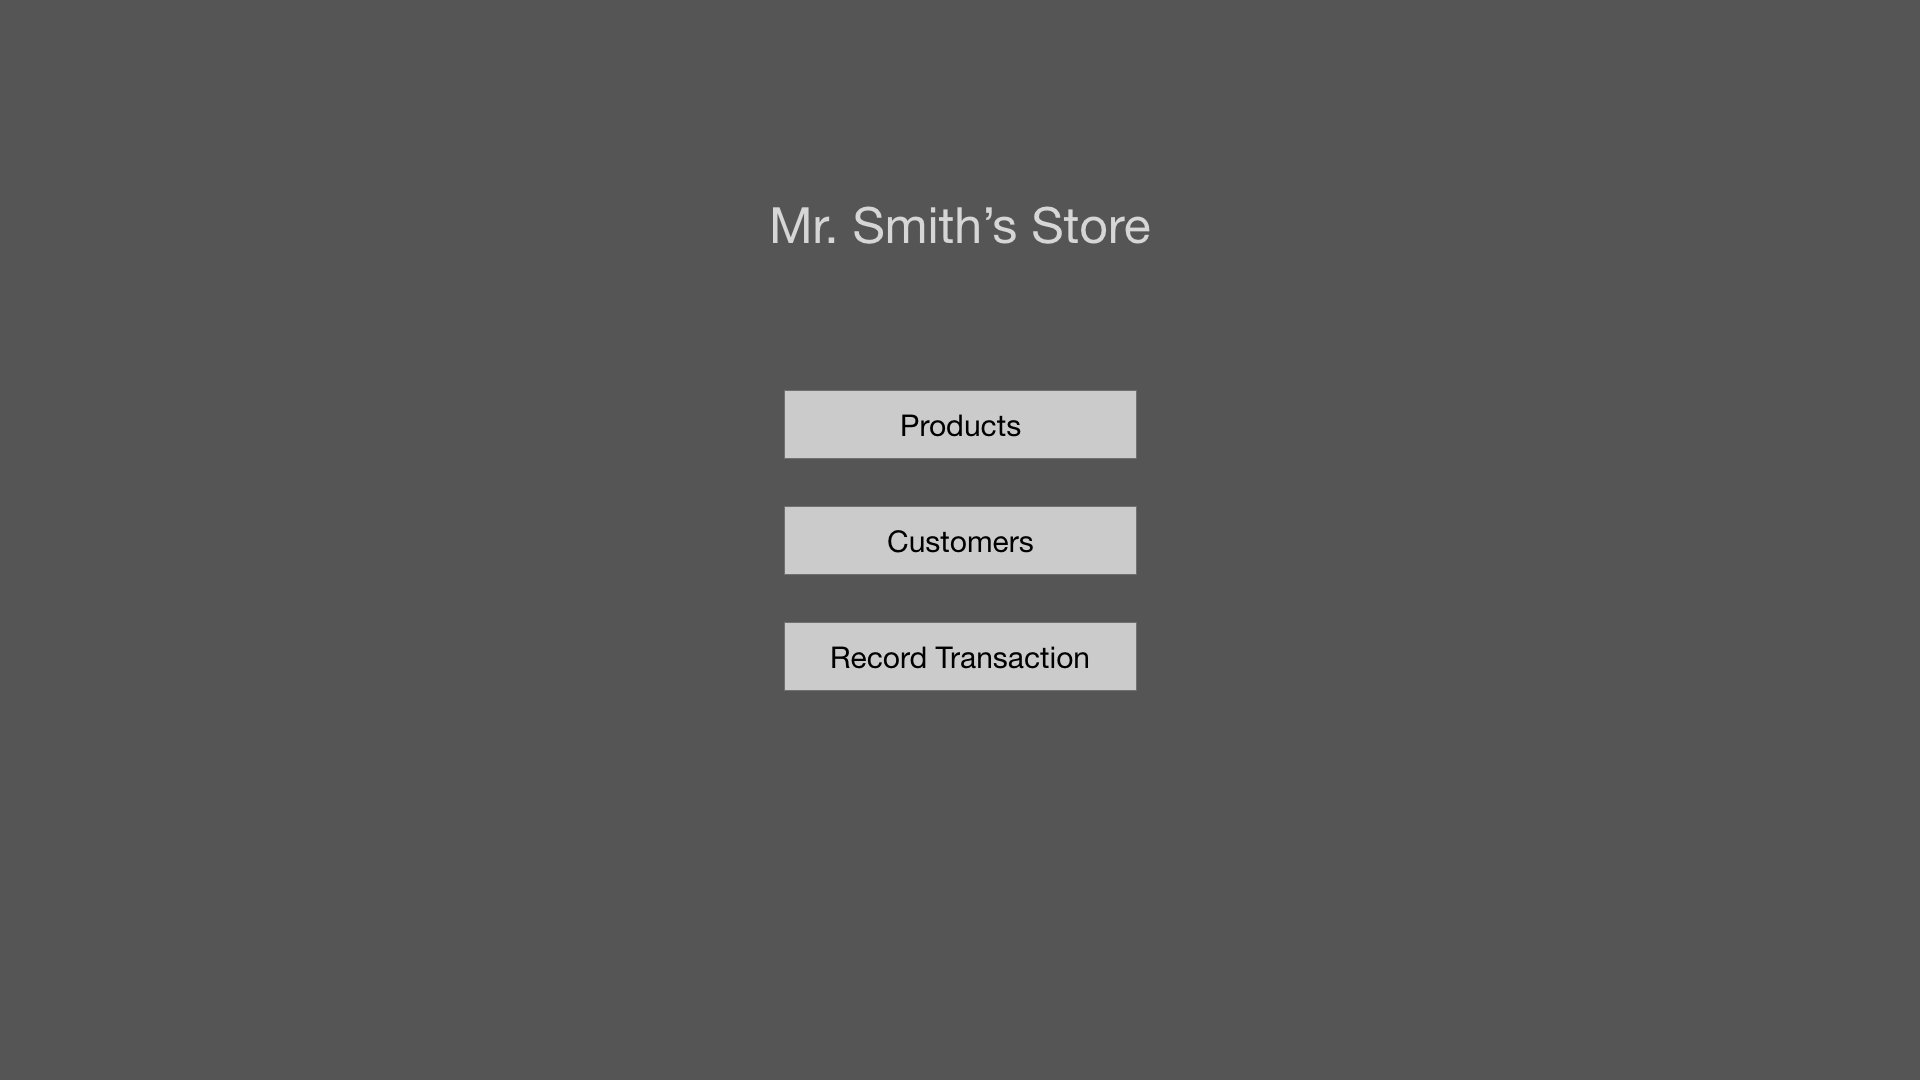
\includegraphics[scale=0.12]{MainMenu}
	\caption{(1)}
	\end{subfigure}%
	\begin{subfigure}{.5\textwidth}
	\centering
	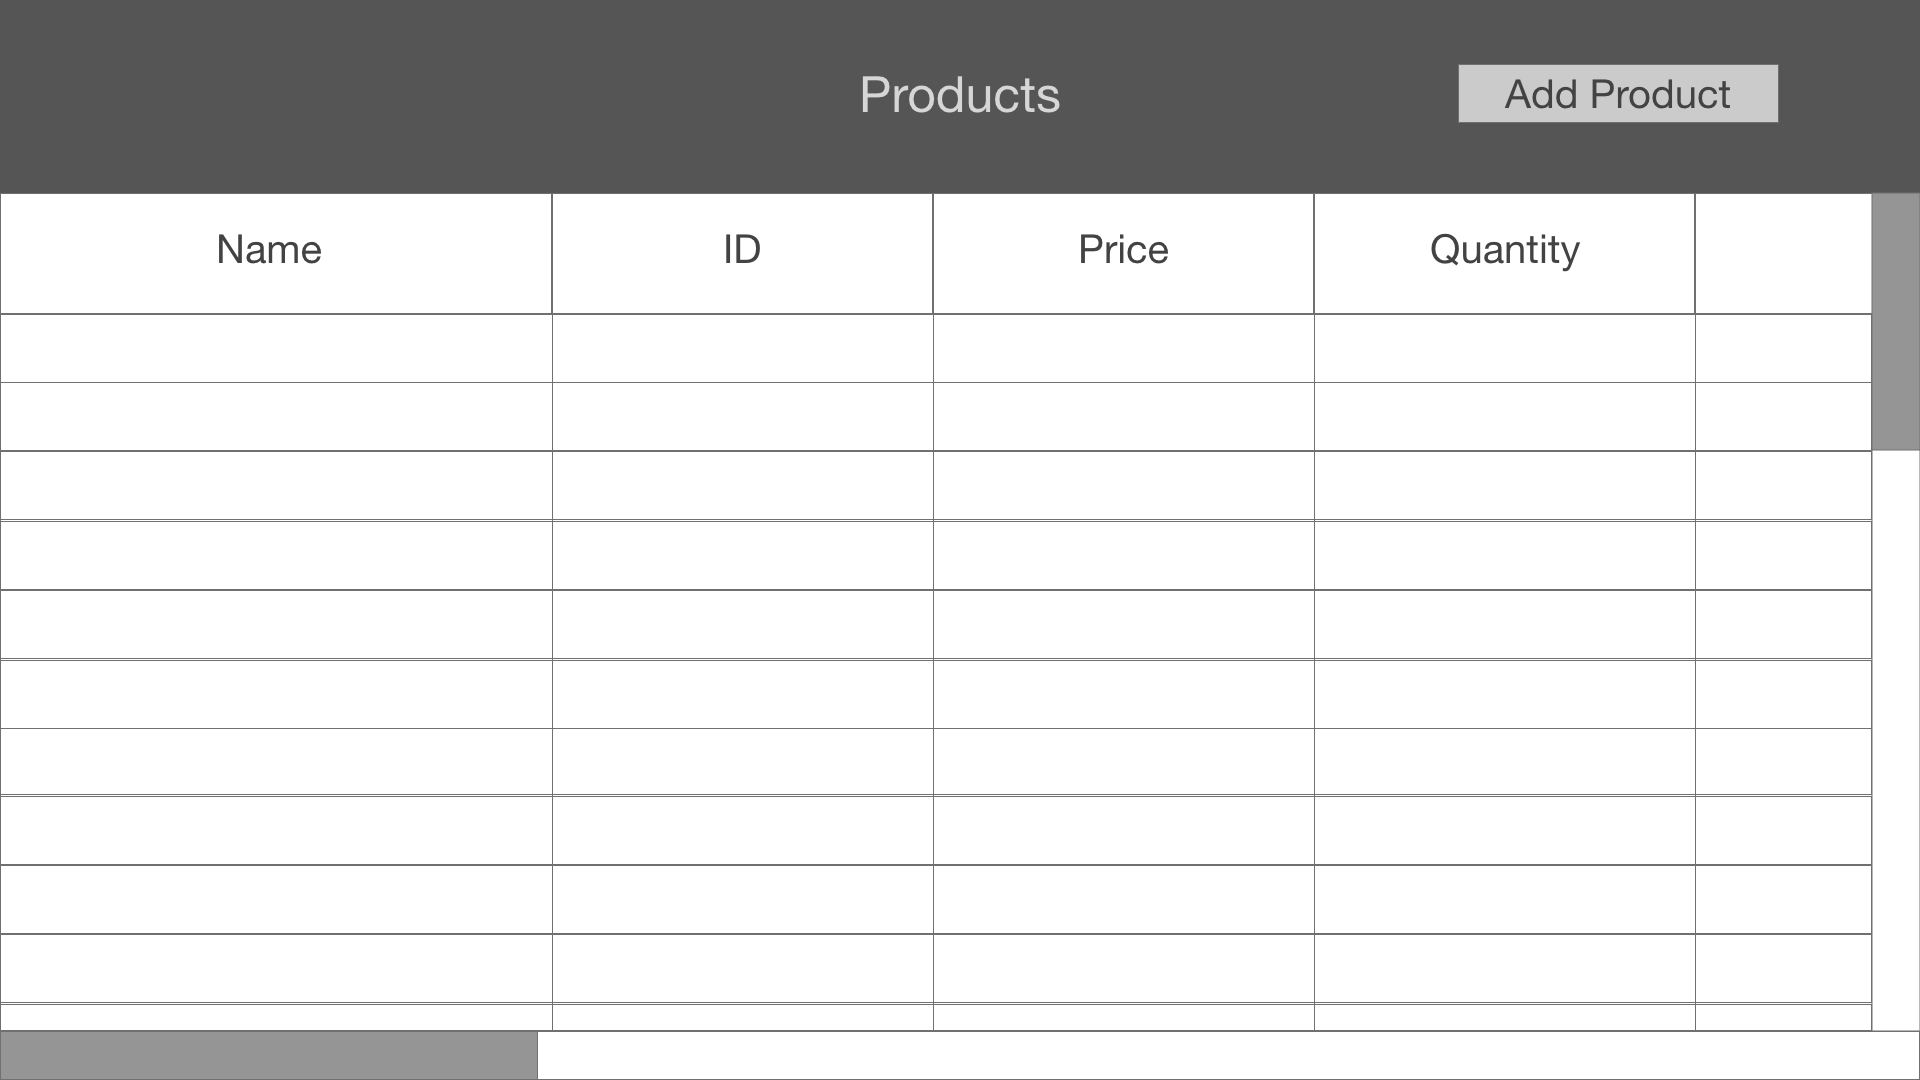
\includegraphics[scale=0.12]{AddProduct}
	\caption{(2)}
	\end{subfigure}
\end{figure}
\begin{figure}[h]
	\begin{subfigure}{.5\textwidth}
	\centering
	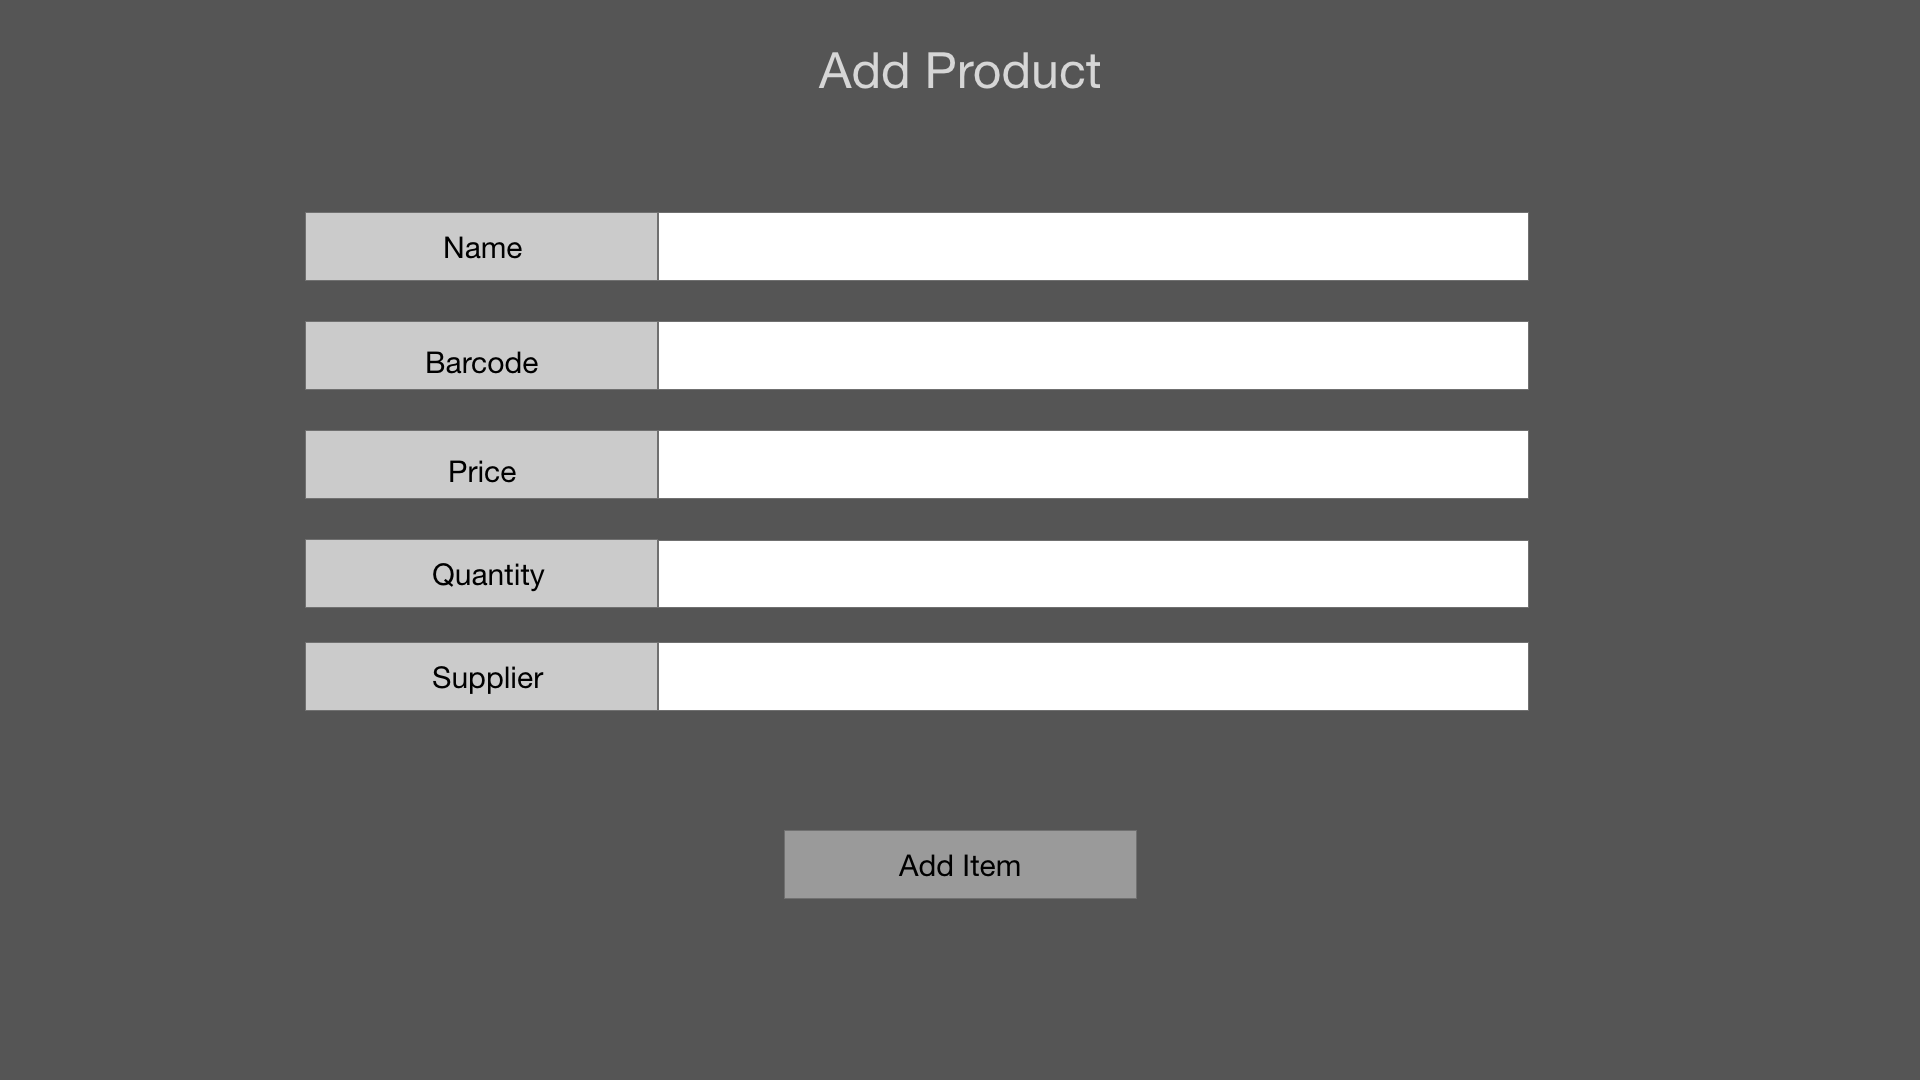
\includegraphics[scale=0.12]{ProdInfo}
	\caption{(3)}
	\end{subfigure}%
	\begin{subfigure}{.5\textwidth}
	\centering
	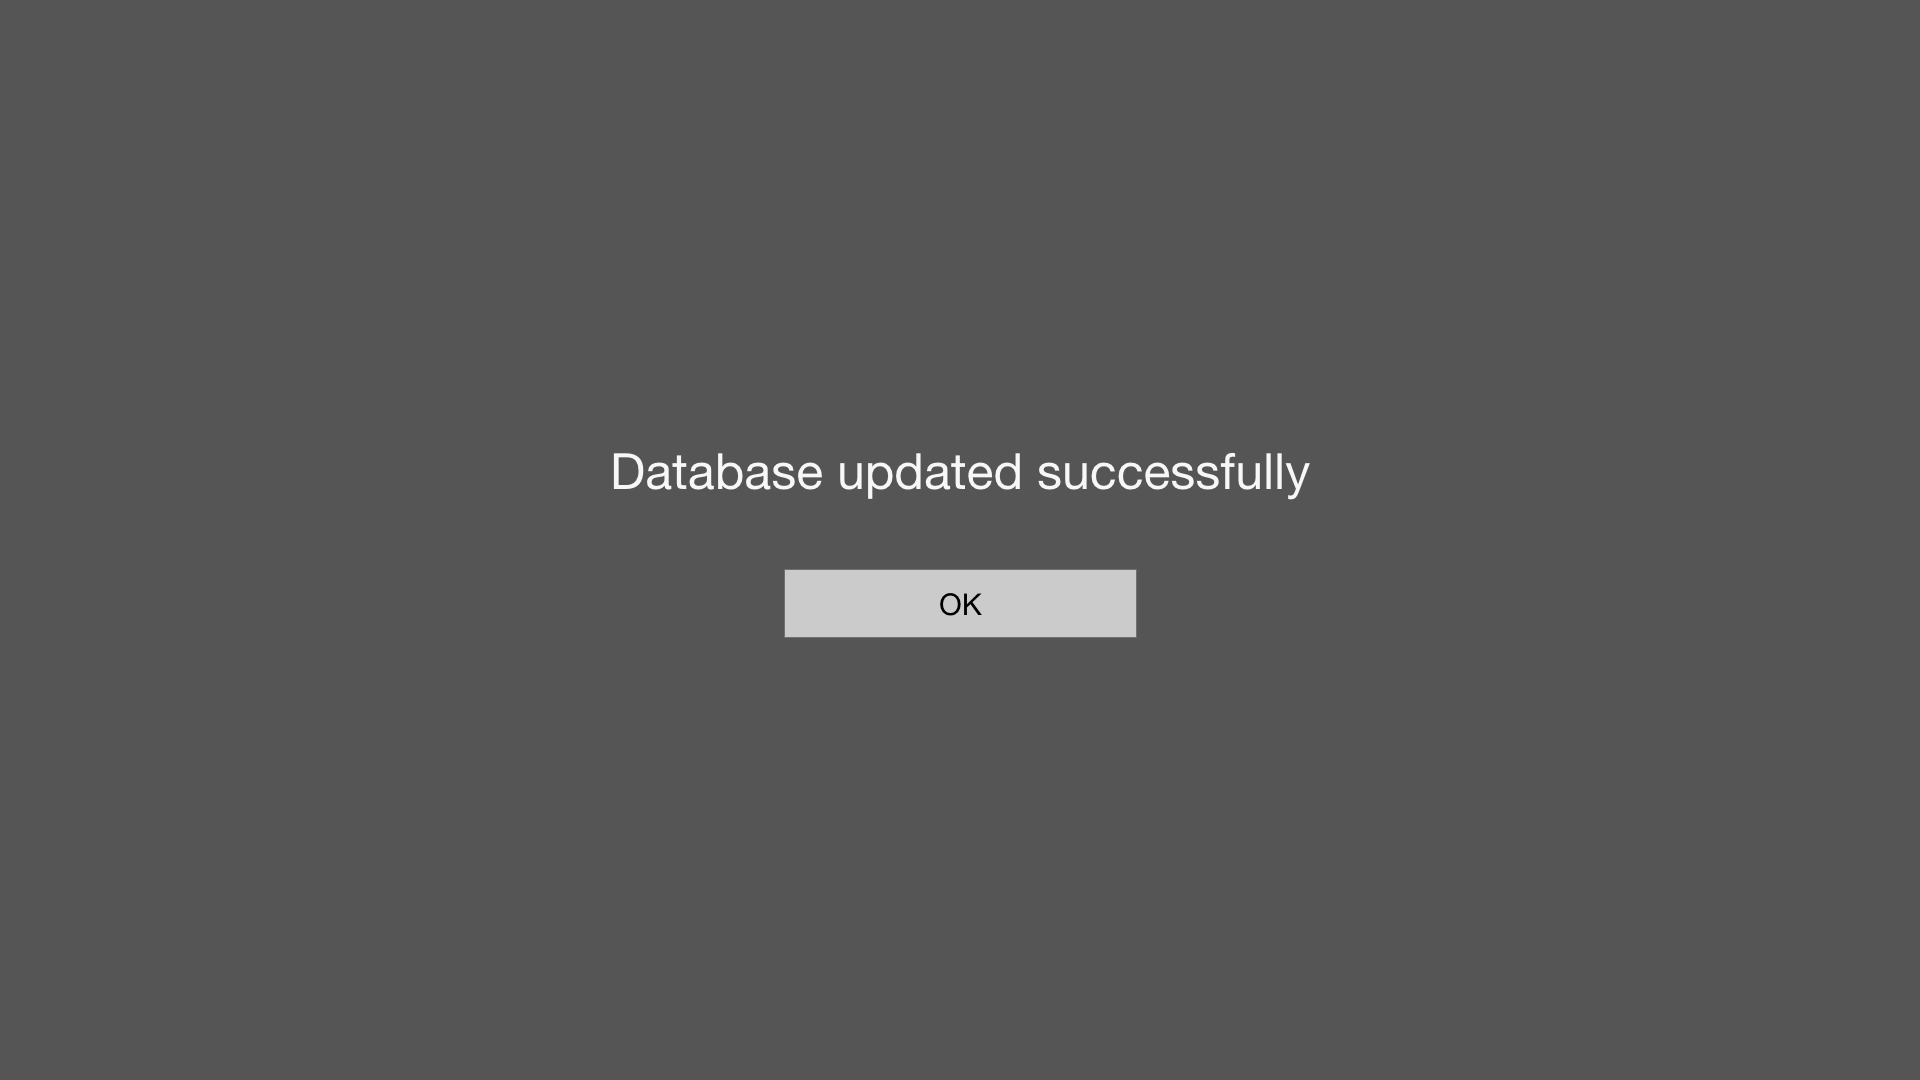
\includegraphics[scale=0.12]{Success}
	\caption{(4)}
	\end{subfigure}
\end{figure}
\newpage
\textbf{Use Case:} update a product in the system\\
\textbf{Actors:} employees\\
\textbf{Goals:} update a product in the database\\
\textbf{Preconditions:} the target product exists in the database\\
\textbf{Postconditions:} the database is updated with desired changes\\
\textbf{steps:}
	\begin{itemize}
		\item[(1)] the user clicks a button to display the product database
		\item[(2)] the system \emph{fetches data from server and} displays the database
		\item the user (double) clicks on the desired field to edit
		\item the system responds by making the field editable
		\item the user enters desired changes and presses enter
		\item the system \sout{updates the underlying database} sends the new product to server
	\end{itemize}
the (1) and (2) views here are the same (1) and (2) views on the previous page

\section{User Story: Add Customer}
	\textbf{Use case:} add a customer into the system\\
	\textbf{Actors:} employees\\
	\textbf{Goals:} update database to include new customer\\
	\textbf{Related use cases:} adding a product or transaction\\
	\textbf{Preconditions, postconditions:} Same as above just replace "product" with "customer"\\
		\textbf{Steps:}
		\begin{itemize}
		\item[(1)] the user clicks a button to display the customer database
		\item[(2)] the system displays the database
		\item the user clicks a plus button 
		\item[(3)] the system displays a screen with text fields for the customer info
		\item the user enters the information and clicks an add button
		\item[(4)] the system \sout{updates the database} \emph{sends data to server} and displays a confirmation message
		\item the user clicks confirm 
		\item[(1)] the system returns to the main menu
		\end{itemize}
\begin{figure}[h]
	\begin{subfigure}{.5\textwidth}
	\centering
	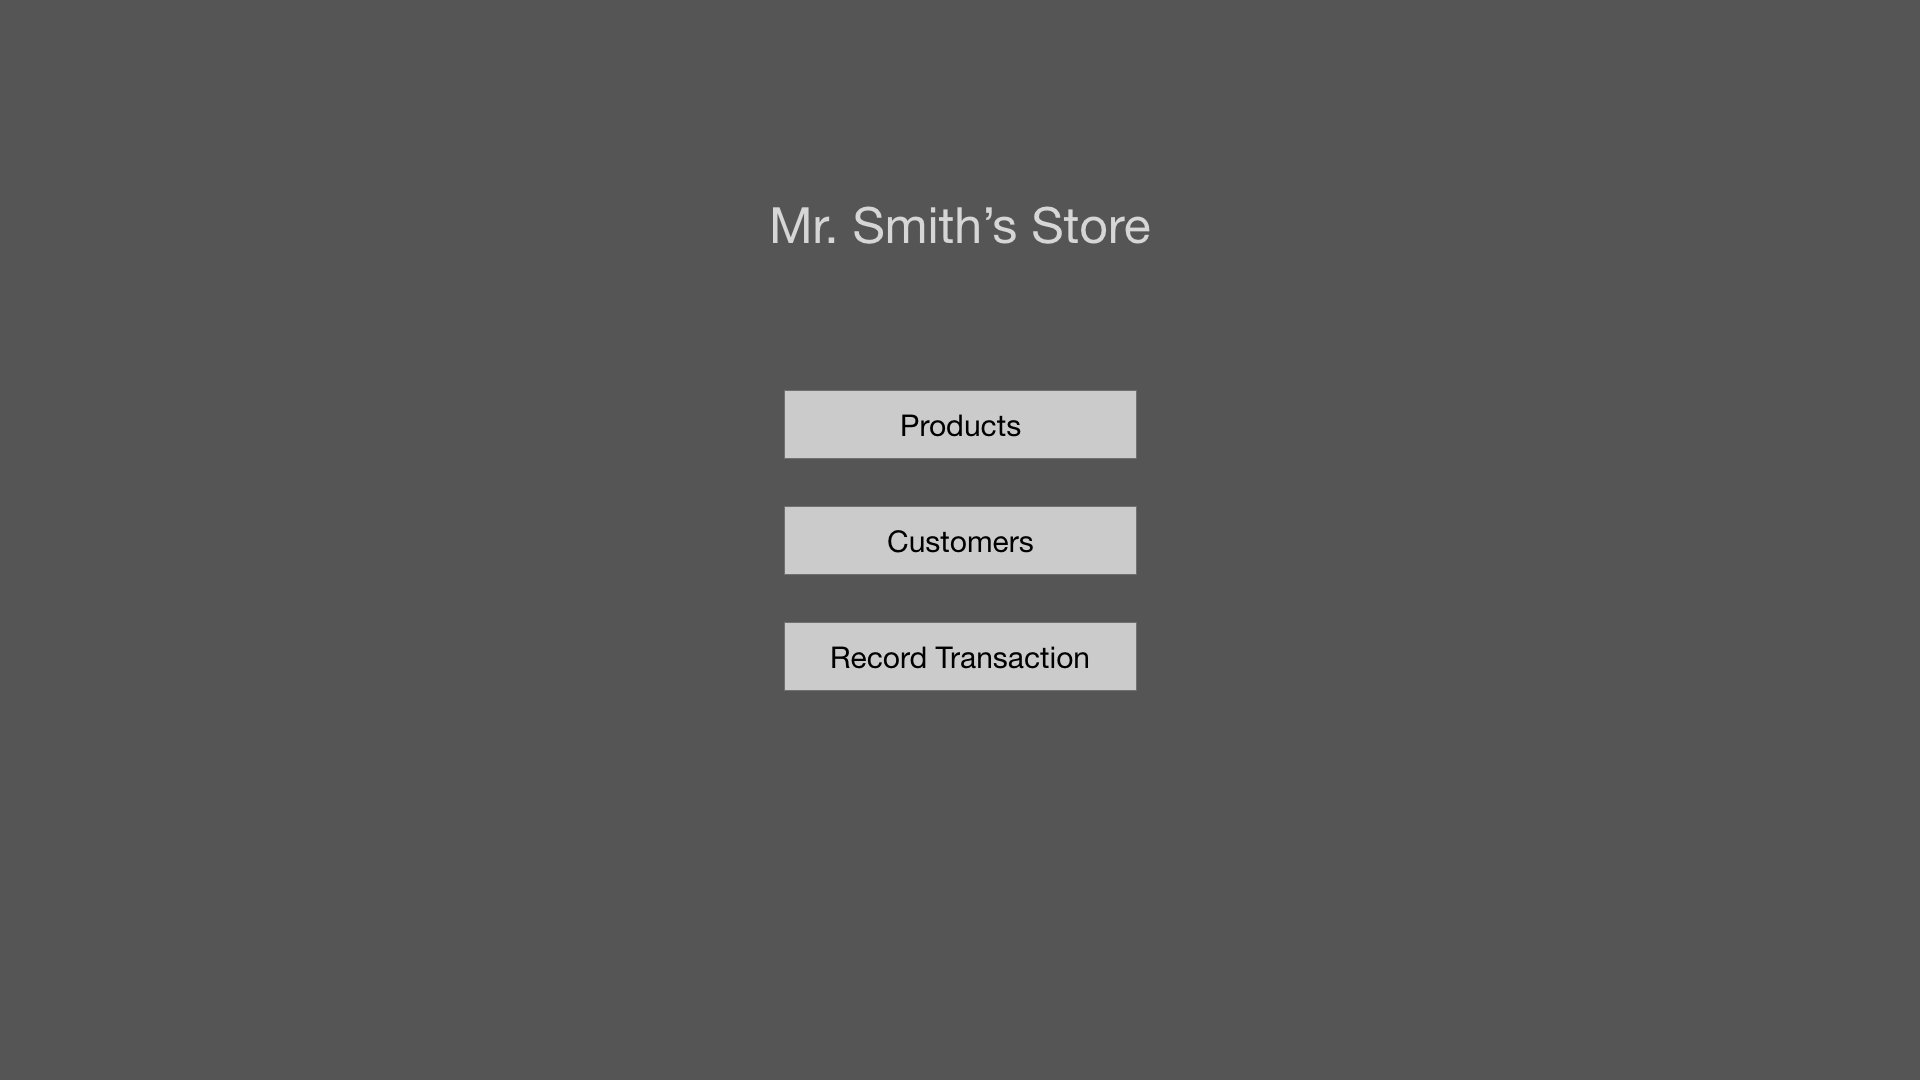
\includegraphics[scale=0.12]{MainMenu}
	\caption{(1)}
	\end{subfigure}%
	\begin{subfigure}{.5\textwidth}
	\centering
	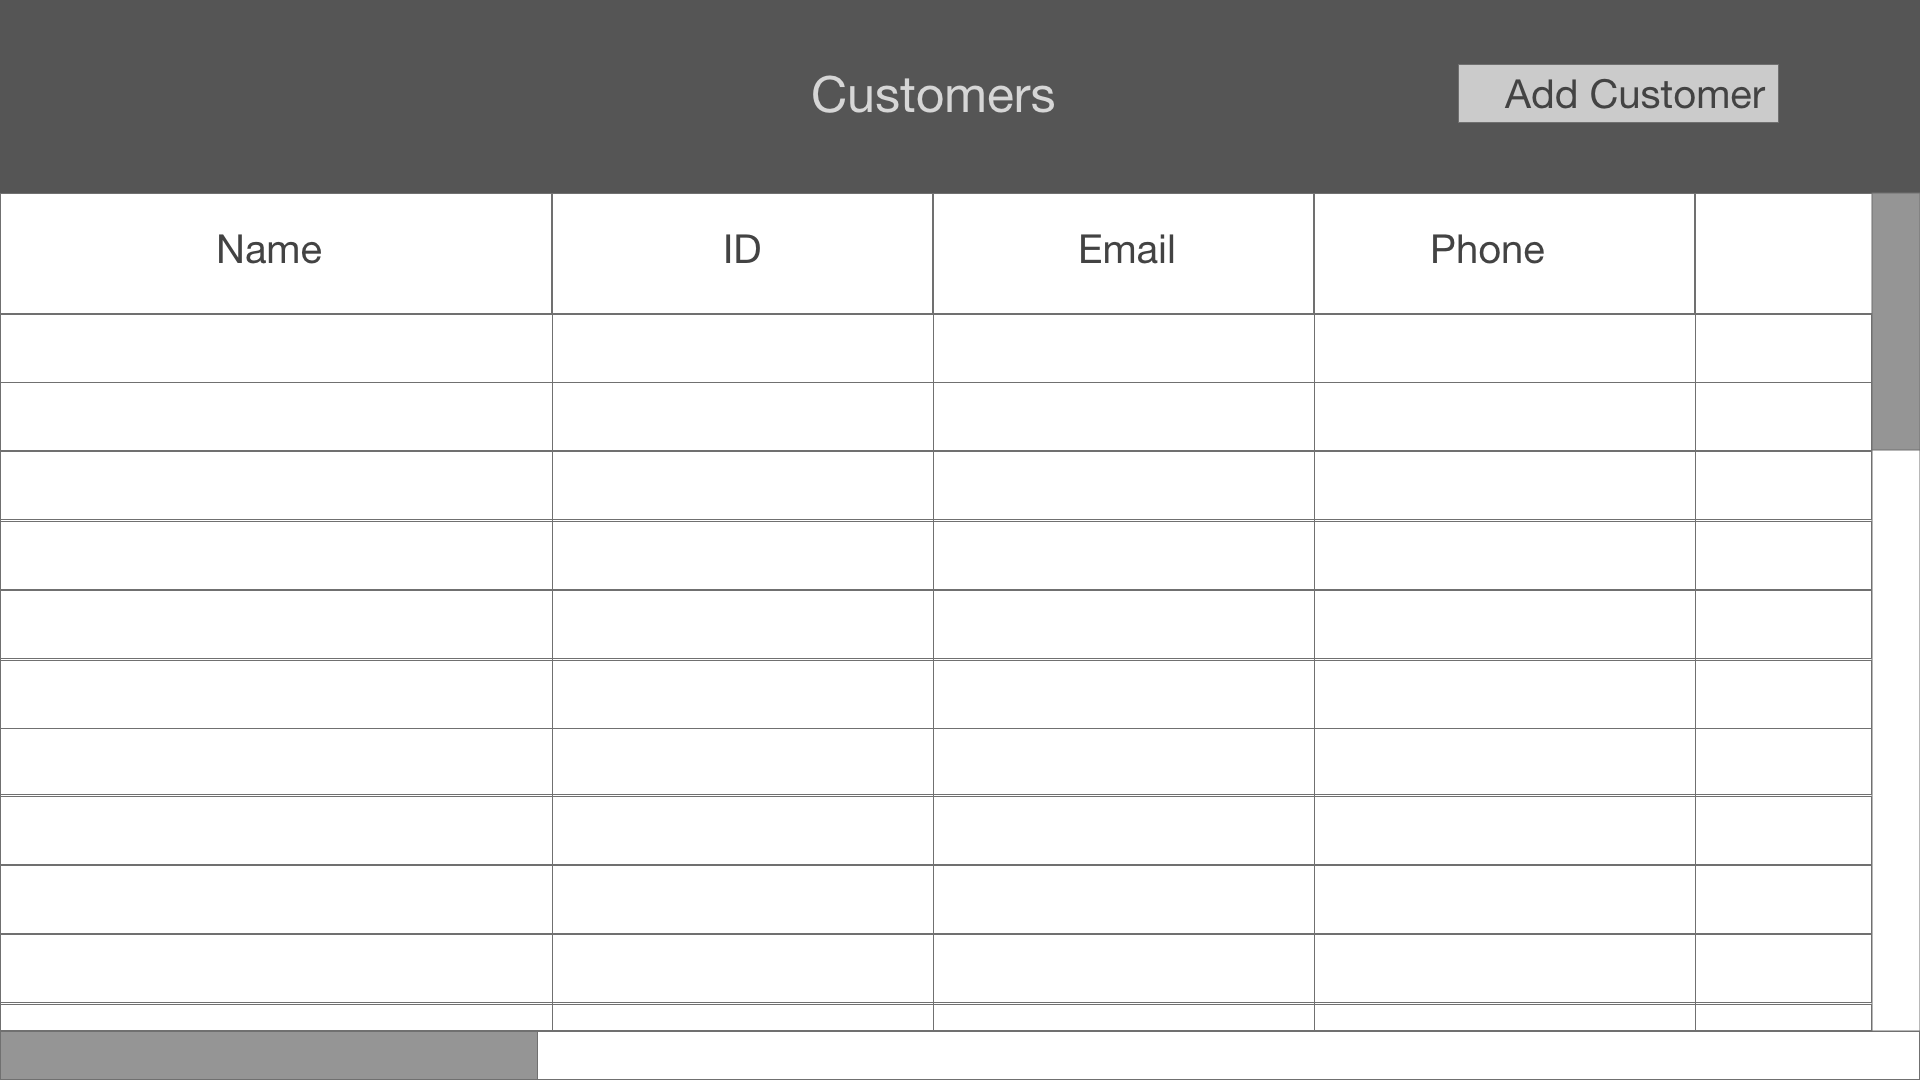
\includegraphics[scale=0.12]{AddCustomer}
	\caption{(2)}
	\end{subfigure}
\end{figure}
\begin{figure}[h]
	\begin{subfigure}{.5\textwidth}
	\centering
	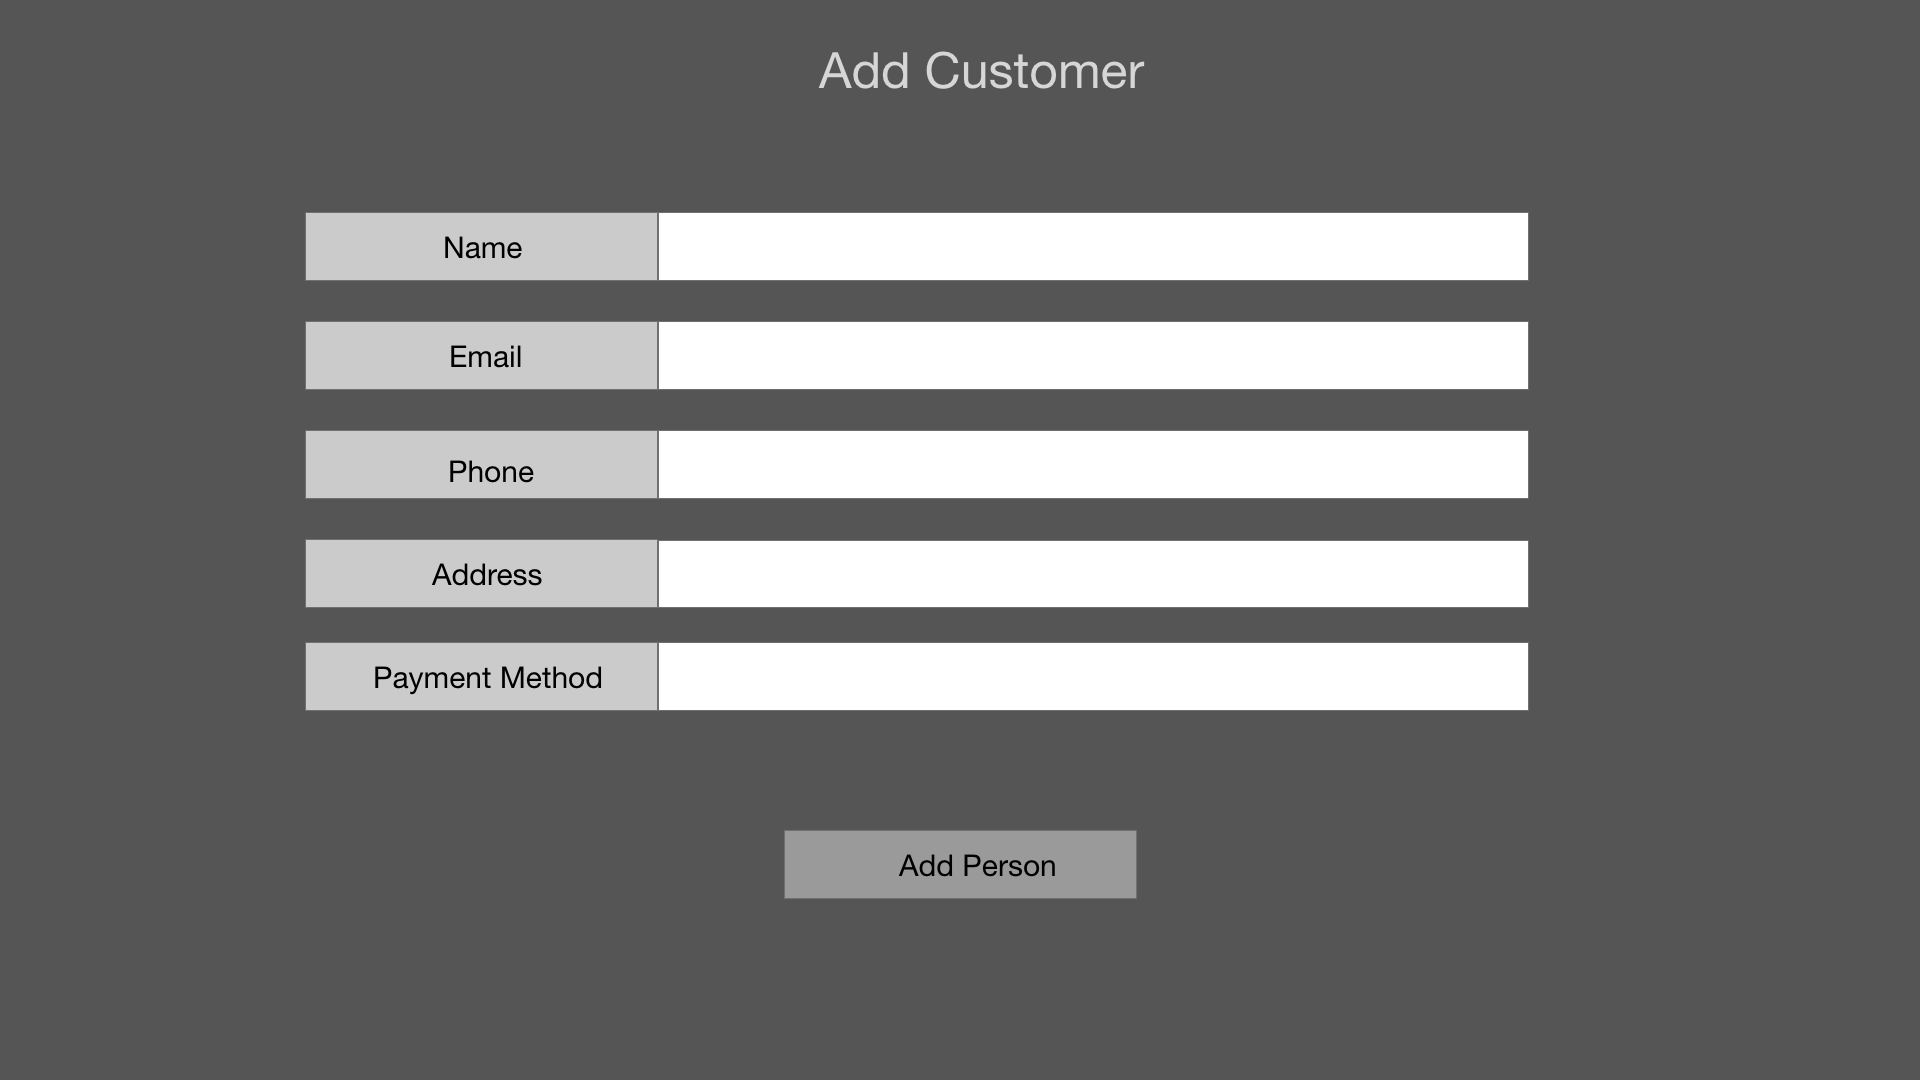
\includegraphics[scale=0.12]{CustInfo}
	\caption{(3)}
	\end{subfigure}%
	\begin{subfigure}{.5\textwidth}
	\centering
	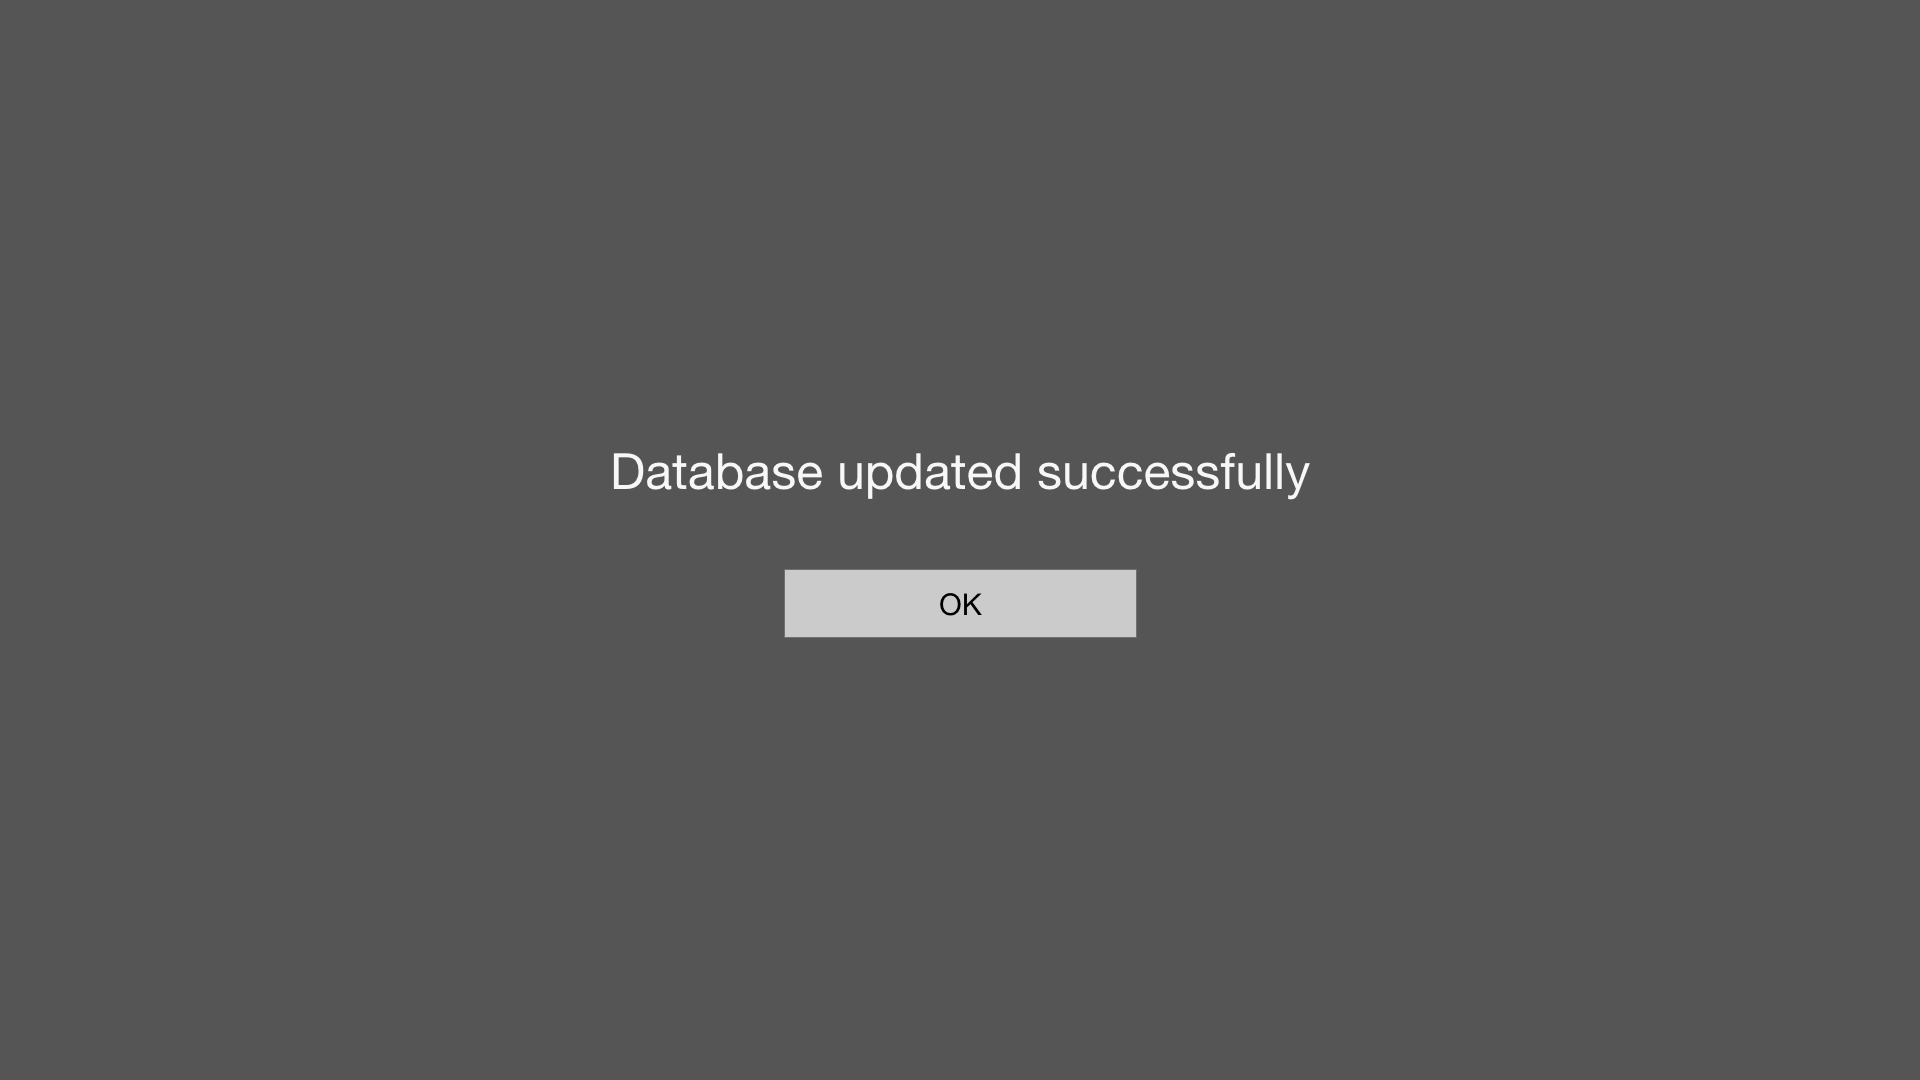
\includegraphics[scale=0.12]{Success}
	\caption{(4)}
	\end{subfigure}
\end{figure}
\newpage
\textbf{Use Case:} update a customer in the system\\
\textbf{Actors:} employees\\
\textbf{Goals:} update a customer entity in the database\\
\textbf{Preconditions:} the specific customer exists in the database \emph{and server is running}\\
\textbf{Postconditions:} the database is updated with desired changes\\
\textbf{steps:}
	\begin{itemize}
		\item[(1)] the user clicks a button to display the customer database
		\item[(2)] the system displays the database
		\item the user (double) clicks on the desired field to edit
		\item the system responds by making the field editable
		\item the user enters desired changes and presses enter
		\item the system \sout{updates the underlying database} \emph{sends info to server}
	\end{itemize}
the (1) and (2) views here are the same (1) and (2) views on the previous page

\section{User Story: Add Transaction}
	\textbf{Use Case:} record a transaction\\
	\textbf{Actors:} employees\\
	\textbf{Goals:} update database to include transaction\\
	\textbf{steps:}
	\begin{itemize}
		\item[(1)] the user clicks a button to record a transaction
		\item[(2)] the system displays a screen with text fields for transaction
		\item the user enters in the information and clicks ok
		\item[(3)] the system displays the receipt with names and prices for confirmation
		\item the user reviews the information and clicks ok
		\item[(4)] the system saves the purchase \sout{to the database} and displays a success message
	\end{itemize}
\begin{figure}[h]
	\begin{subfigure}{.5\textwidth}
	\centering
	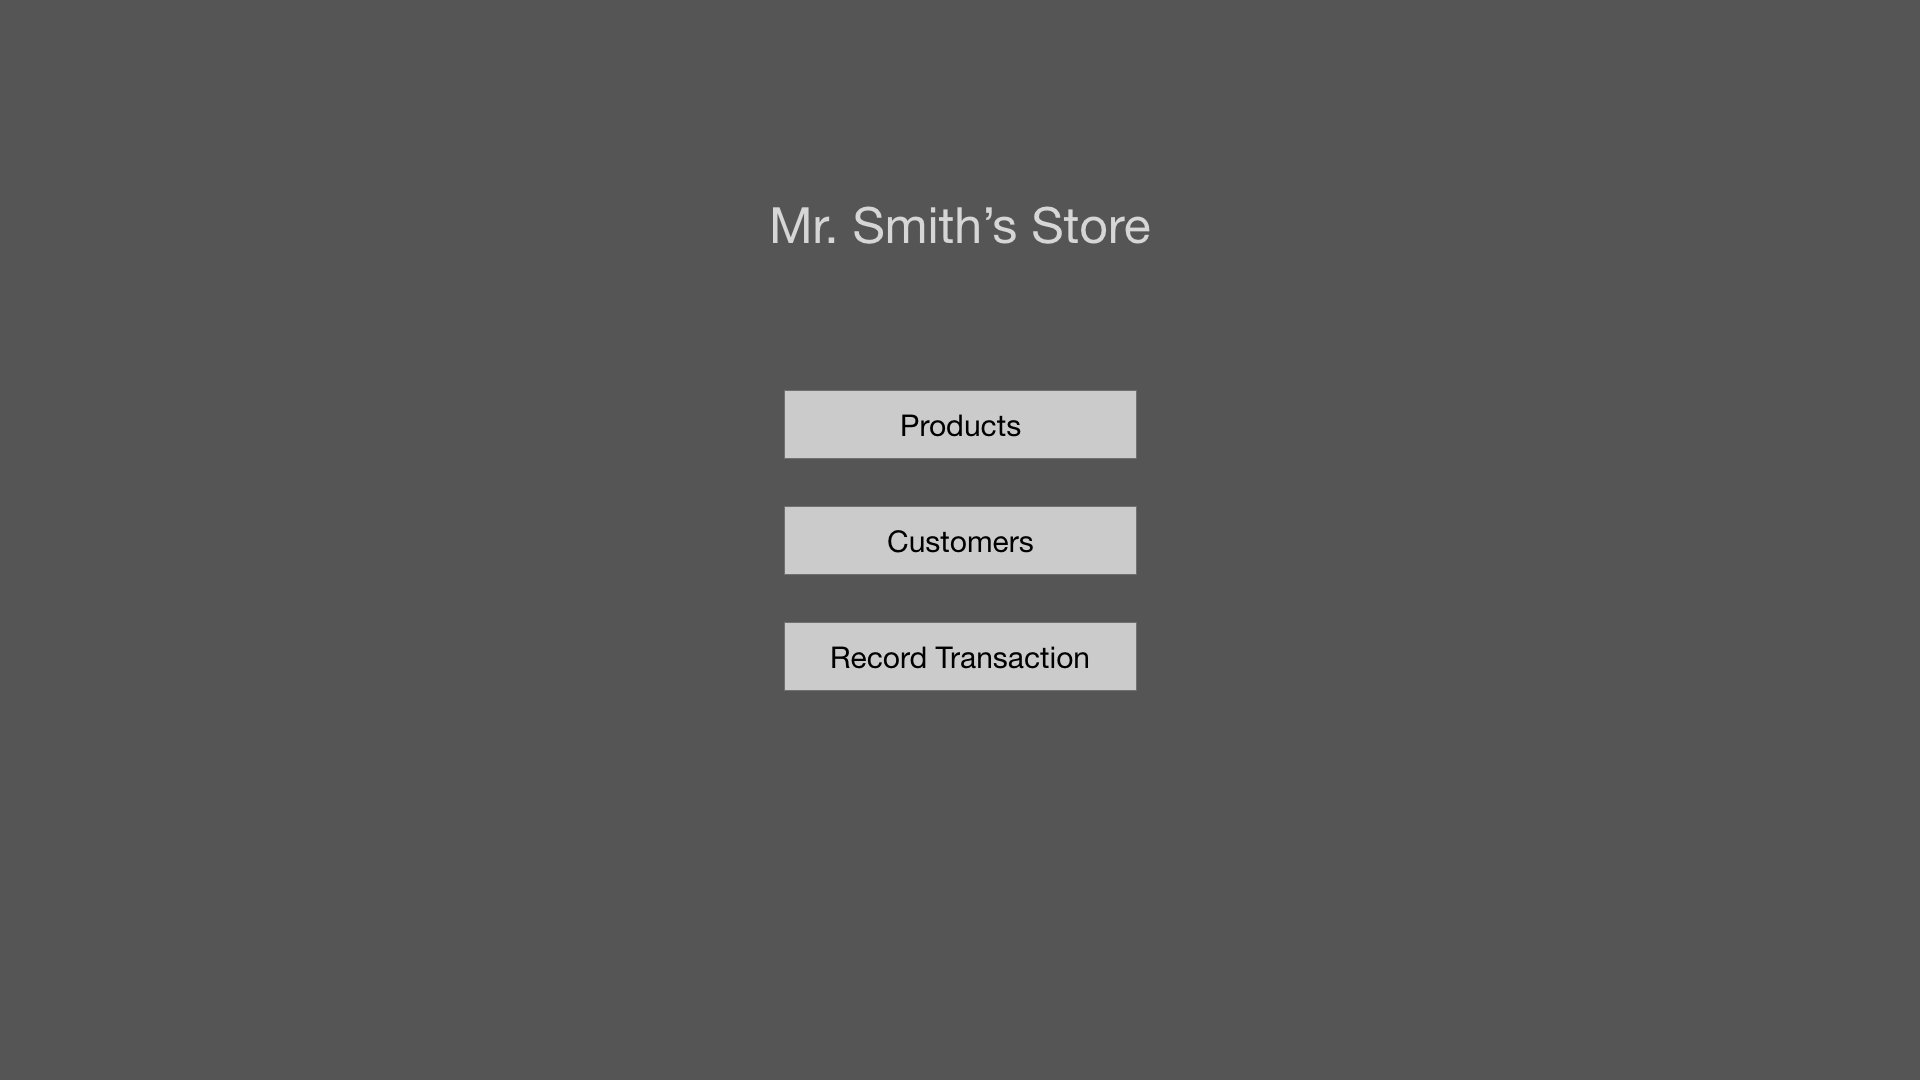
\includegraphics[scale=0.12]{MainMenu}
	\caption{(1)}
	\end{subfigure}%
	\begin{subfigure}{.5\textwidth}
	\centering
	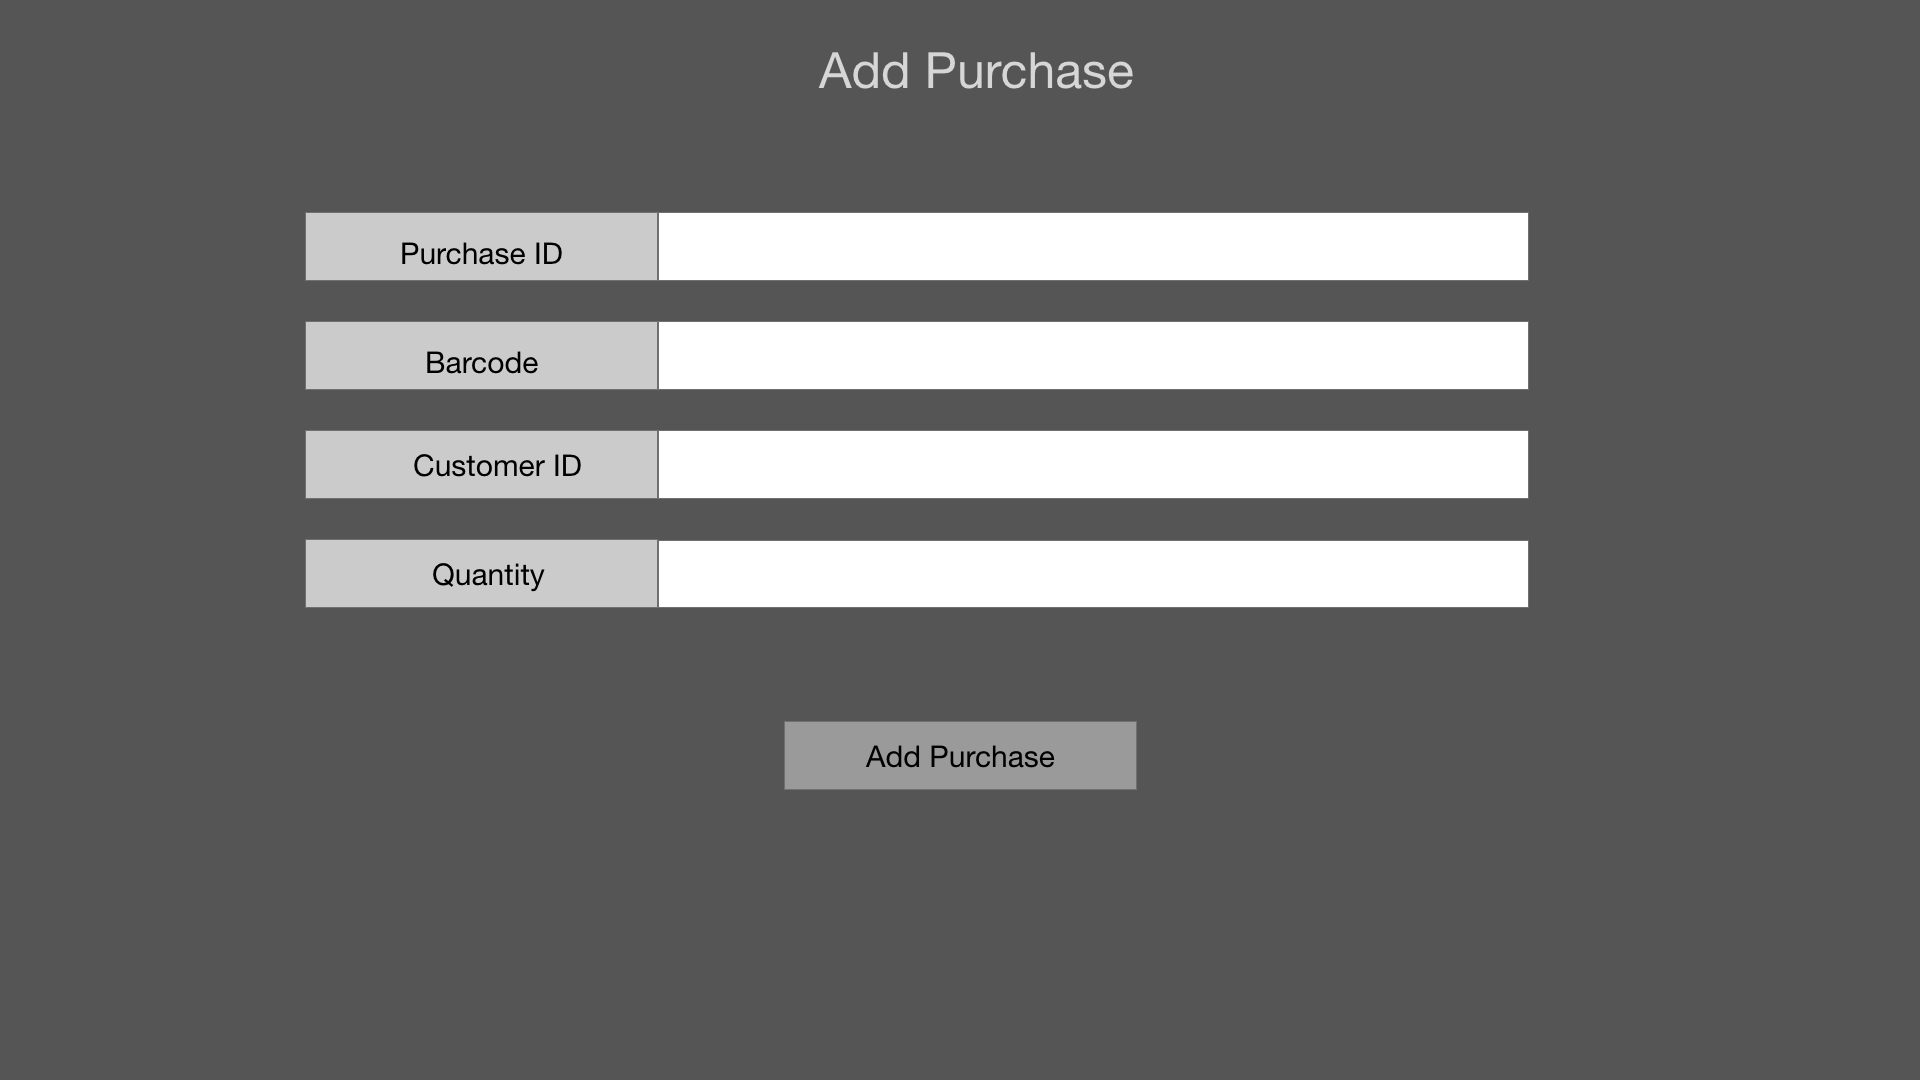
\includegraphics[scale=0.12]{AddPurchase}
	\caption{(2)}
	\end{subfigure}
\end{figure}
\begin{figure}[h]
	\begin{subfigure}{.5\textwidth}
	\centering
	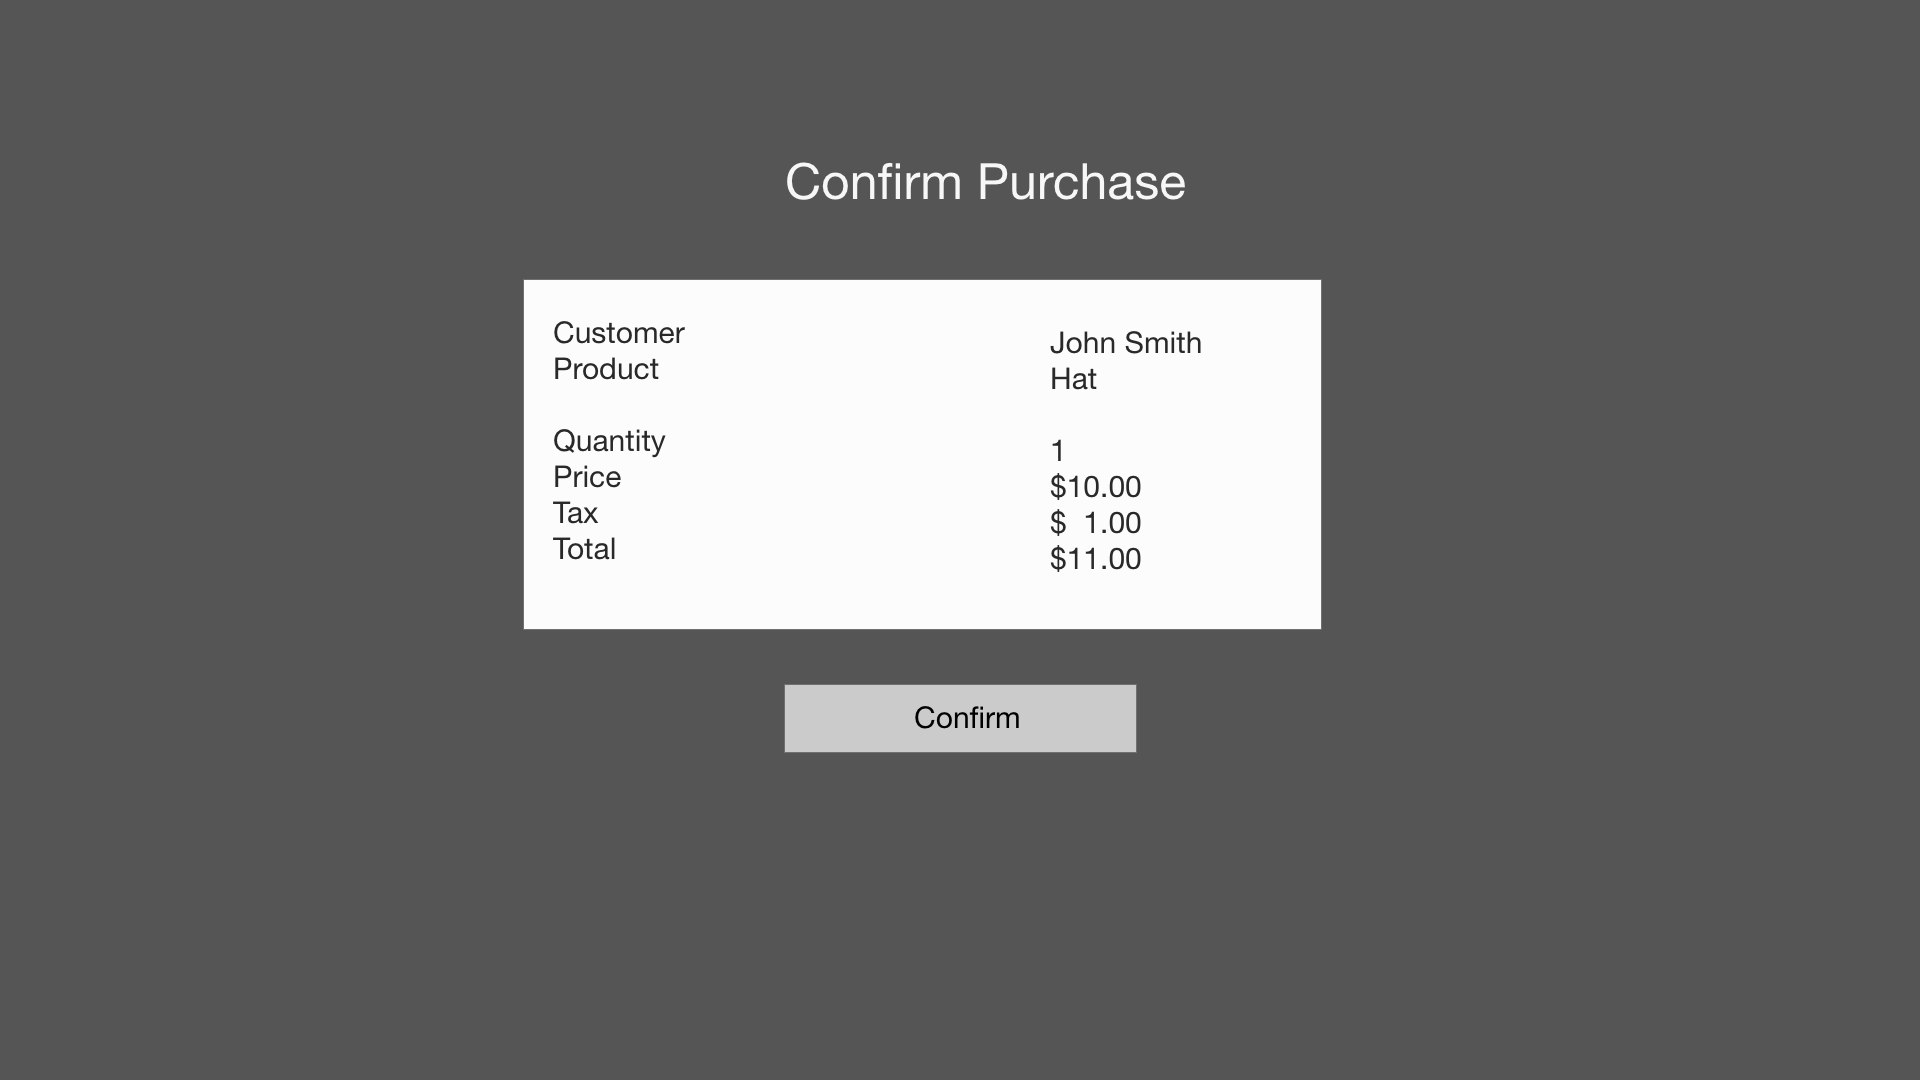
\includegraphics[scale=0.12]{PurchaseConfirm}
	\caption{(3)}
	\end{subfigure}%
	\begin{subfigure}{.5\textwidth}
	\centering
	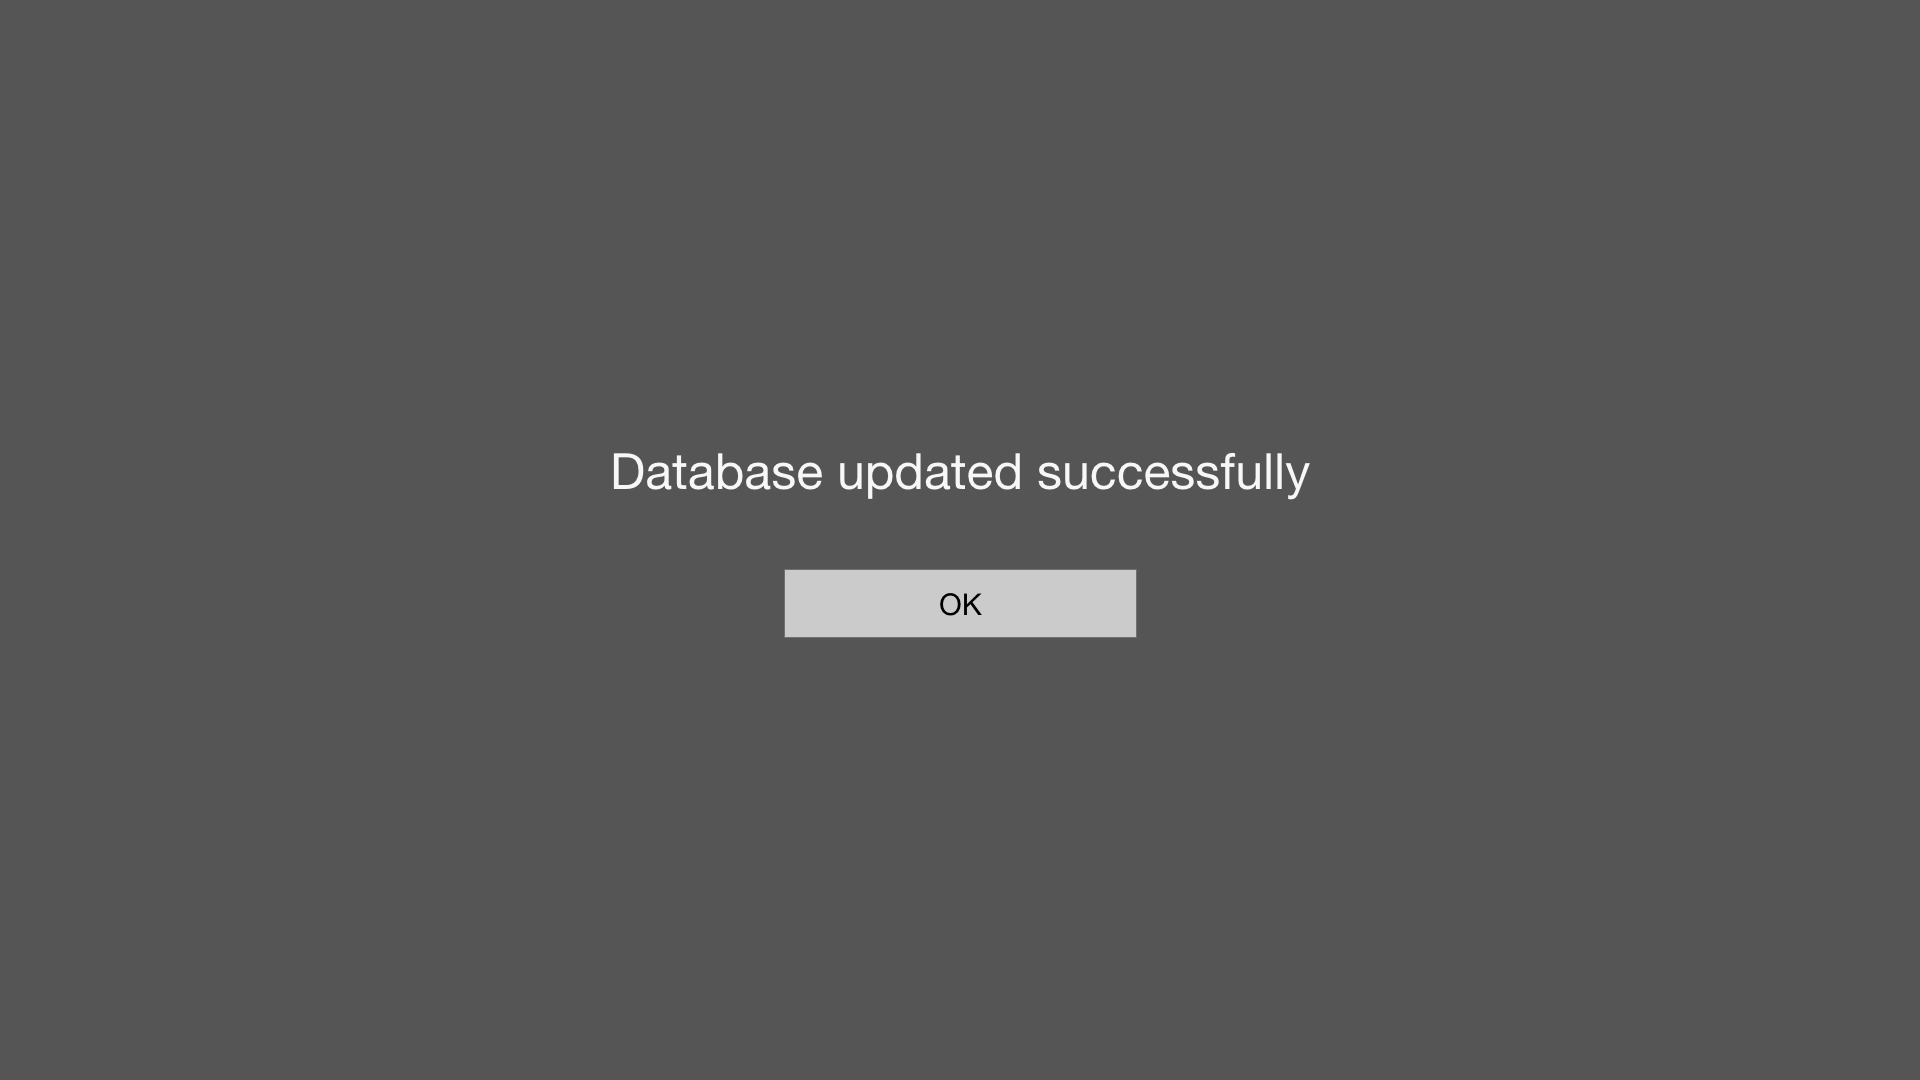
\includegraphics[scale=0.12]{Success}
	\caption{(4)}
	\end{subfigure}
\end{figure}
	\textbf{Use Case:} refund (delete) a transaction\\
	\textbf{Actors:} employees\\
	\textbf{Goals:} delete purchase from database\\
	\textbf{steps:}
	\begin{itemize}
		\item[(1)] the user clicks a button to view transaction database
		\item[(2)] the system displays the purchase database
		\item the user right clicks (or something) on a purchase to delete it
		\item[(3)] the system displays the purchase receipt with a button to delete
		\item the user clicks the delete button
		\item[(2)] the system removes the purchase \sout{from the database} and updates the view
	\end{itemize}
	Same views as above except the (1) view (main menu) includes a "view transaction" button.
\newpage
\begin{center} SQL code \end{center}
\Suppressnumber
\begin{lstlisting}
CREATE TABLE Customers (
	"CustomerID" INTEGER NOT NULL UNIQUE,
	"Name" TEXT,
	"Email" TEXT,
	"Phone" TEXT,
	"Address" TEXT,
	"PaymentInfo" TEXT,
	PRIMARY KEY("CustomerID")
);

CREATE TABLE Products (
	"Barcode" INTEGER NOT NULL UNIQUE,
	"Name" TEXT,
	"Price" REAL,
	"Supplier" TEXT,
	"Quantity" INTEGER,
	PRIMARY KEY("Barcode")
);

CREATE TABLE Purchases (
	PurchaseID INTEGER NOT NULL UNIQUE,
	CustomerID INTEGER,
	ProductID INTEGER,
	Price REAL,
	Tax REAL,
	Cost REAL,
	Date TEXT,
	Quantity INTEGER,
	PRIMARY KEY("PurchaseID"),
	FOREIGN KEY("CustomerID") REFERENCES Customers(CustomerID),
	FOREIGN KEY("Barcode") REFERENCES Products(Barcode)
);

CREATE TABLE IF NOT EXISTS User (
	Username text,
	Password text,
	UserType integer,
	CustomerID integer
);

INSERT INTO Customers (CustomerID, Name, Email, Phone, Address, PaymentInfo)
VALUES	(1, 'Alice Appleton', 'aappleton@yahoo.com', '334-555-6123', 
		'345 Apple St', 'credit card'),
			(2, 'Bob Baker', 'bbaker@gmail.com', '123-456-7891', 
		'123 Abbey Rd', 'paypal'),
			(3, 'Charlie Wilson', 'cwilson@outlook.com', '453-674-1235', 
		'7351 Ross St', 'cash'),
			(4, 'Dan Glover', 'dglover@gmail.com', '954-102-6423', 
		'123 Main St', 'credit card'),
			(5, 'Eve Mcgee', 'emcgee@icloud.com', '121-644-1345', 
		'101 College St', 'credit card');

INSERT INTO Products (Barcode, Name, Price, Supplier, Quantity)
VALUES	(1, 'jacket', 59.99, 'Jackets Inc.', 10),
			(2, 'pants', 21.95, 'Nike', 25),
			(3, 't-shirt', 14.99, 'Old Navy', 100),
			(4, 'dress', 44.95, 'Dress store', 30),
			(5, 'shoes', 49.99, 'Shoemart', 15);

INSERT INTO Purchases (PurchaseID, CustomerID, Barcode, Price, Tax, Cost, 
	Date, Quantity)
VALUES	(1, 3, 2, 21.95, 0.05, 22.00, '10/4/2019', 1),
			(2, 5, 5, 41.55, 1.00, 42.55, '10/5/2019', 1),
			(3, 4, 5, 49.99, 0.00, 99.98, '10/6/2019', 2),
			(4, 2, 1, 59.99, 0.01, 60.00, '10/7/2019', 1),
			(5, 5, 2, 24.99, 5.00, 29.99, '10/7/2019', 1),
			(6, 3, 4, 44.95, 3.00, 47.95, '10/8/2019', 1),
			(7, 3, 3, 10.83, 1.00, 11.83, '10/9/2019', 1),
			(8, 1, 2, 21.95, 3.00, 24.95, '10/9/2019', 1),
			(9, 4, 5, 49.99, 0.01, 50.00, '10/10/2019', 1),
			(10, 1, 1, 51.12, 3.00, 54.12, '10/11/2019', 1);
			
INSERT INTO User (Username, Password, UserType, CustomerID) 
VALUES ('admin', 'admin', 0, 0)
		('manager', 'manager', 1, 0)
		('cashier', 'cashier', 2, 0)
		('alice', 'alice', 3, 1)
		('bob', 'password', 3, 2);

\end{lstlisting}
\end{document}